%------------------------------------------------

\begin{fullwidth}

% What is data cleaning
Raw data files may be received in a variety of formats, 
and are often not easy to handle using statistical software.
The tasks described in this chapter have many different names.
Some say data cleaning, others data munging, or maybe data wrangling.
But they all mean the same thing:
transforming raw data into a more convenient format for your intended use.
This is the most time-consuming step of a project's data work, 
particularly when primary data is involved.
It is also essential for data quality. 
This chapter outlines the workflow our team developed to make the process efficient and transparent.
One key point of this workflow is that no changes be made to the contents of data at this point.
Creating new variables, imputing values and correcting outliers
are research decisions.
To make data processing less error-prone,
such changes to the data will be made at a separate stage.
Therefore, the clean dataset,
which is the main output from the tasks discussed in this chapter,
contains almost exactly same information as the raw data,
but in a format that is easier to handle. 

% Chapter overview
The following sections describe the different tasks involved in making newly acquired data ready for analysis.
The first section will show how to make your data \textit{tidy}.
This means adjusting how the dataset is organized until the relationship between its rows and columns is well-defined.
The second section describes quality assurance checks, 
which are necessary to verify the accuracy of your data.
After that, identifying information is typically no longer needed,
therefore the third section outlines steps to remove direct identifiers.
Finally, the last section discusses how to explore each variable in your dataset and 
make sure that it is as well documented and as easy to use as possible.

\end{fullwidth}

%------------------------------------------------


\section{Identifying the identifier(s)}

% Intro
The very first step in creating analysis-friendly datasets
is understanding the data acquired,
and translating this understanding into an intuitive format.
This section discusses what steps may be needed to make sure that each row
in a tabular dataset\sidenote{\textbf{Tabular data:}
	data that is structured into rows and columns. 
	Also called ``rectangular data''.
	Examples of non-rectangular data are a text, or files, such as images.} 
represents one observation.
This may seem trivial, but should not be taken for granted.
Getting to such a format may be harder than expected,
and the \textbf{unit of observation}\sidenote{\textbf{Unit of observation:}
	the unit described by the data. In datasets, it is ideally what each row represents. \url{
		https://dimewiki.worldbank.org/wiki/Unit_of_Observation}}
 may be ambiguous in many raw datasets.
In this section, we will discuss the ideal format to handle data,
which we call a \textit{tidy} format.

\begin{fullwidth}
	\begin{figure}
		\centering
		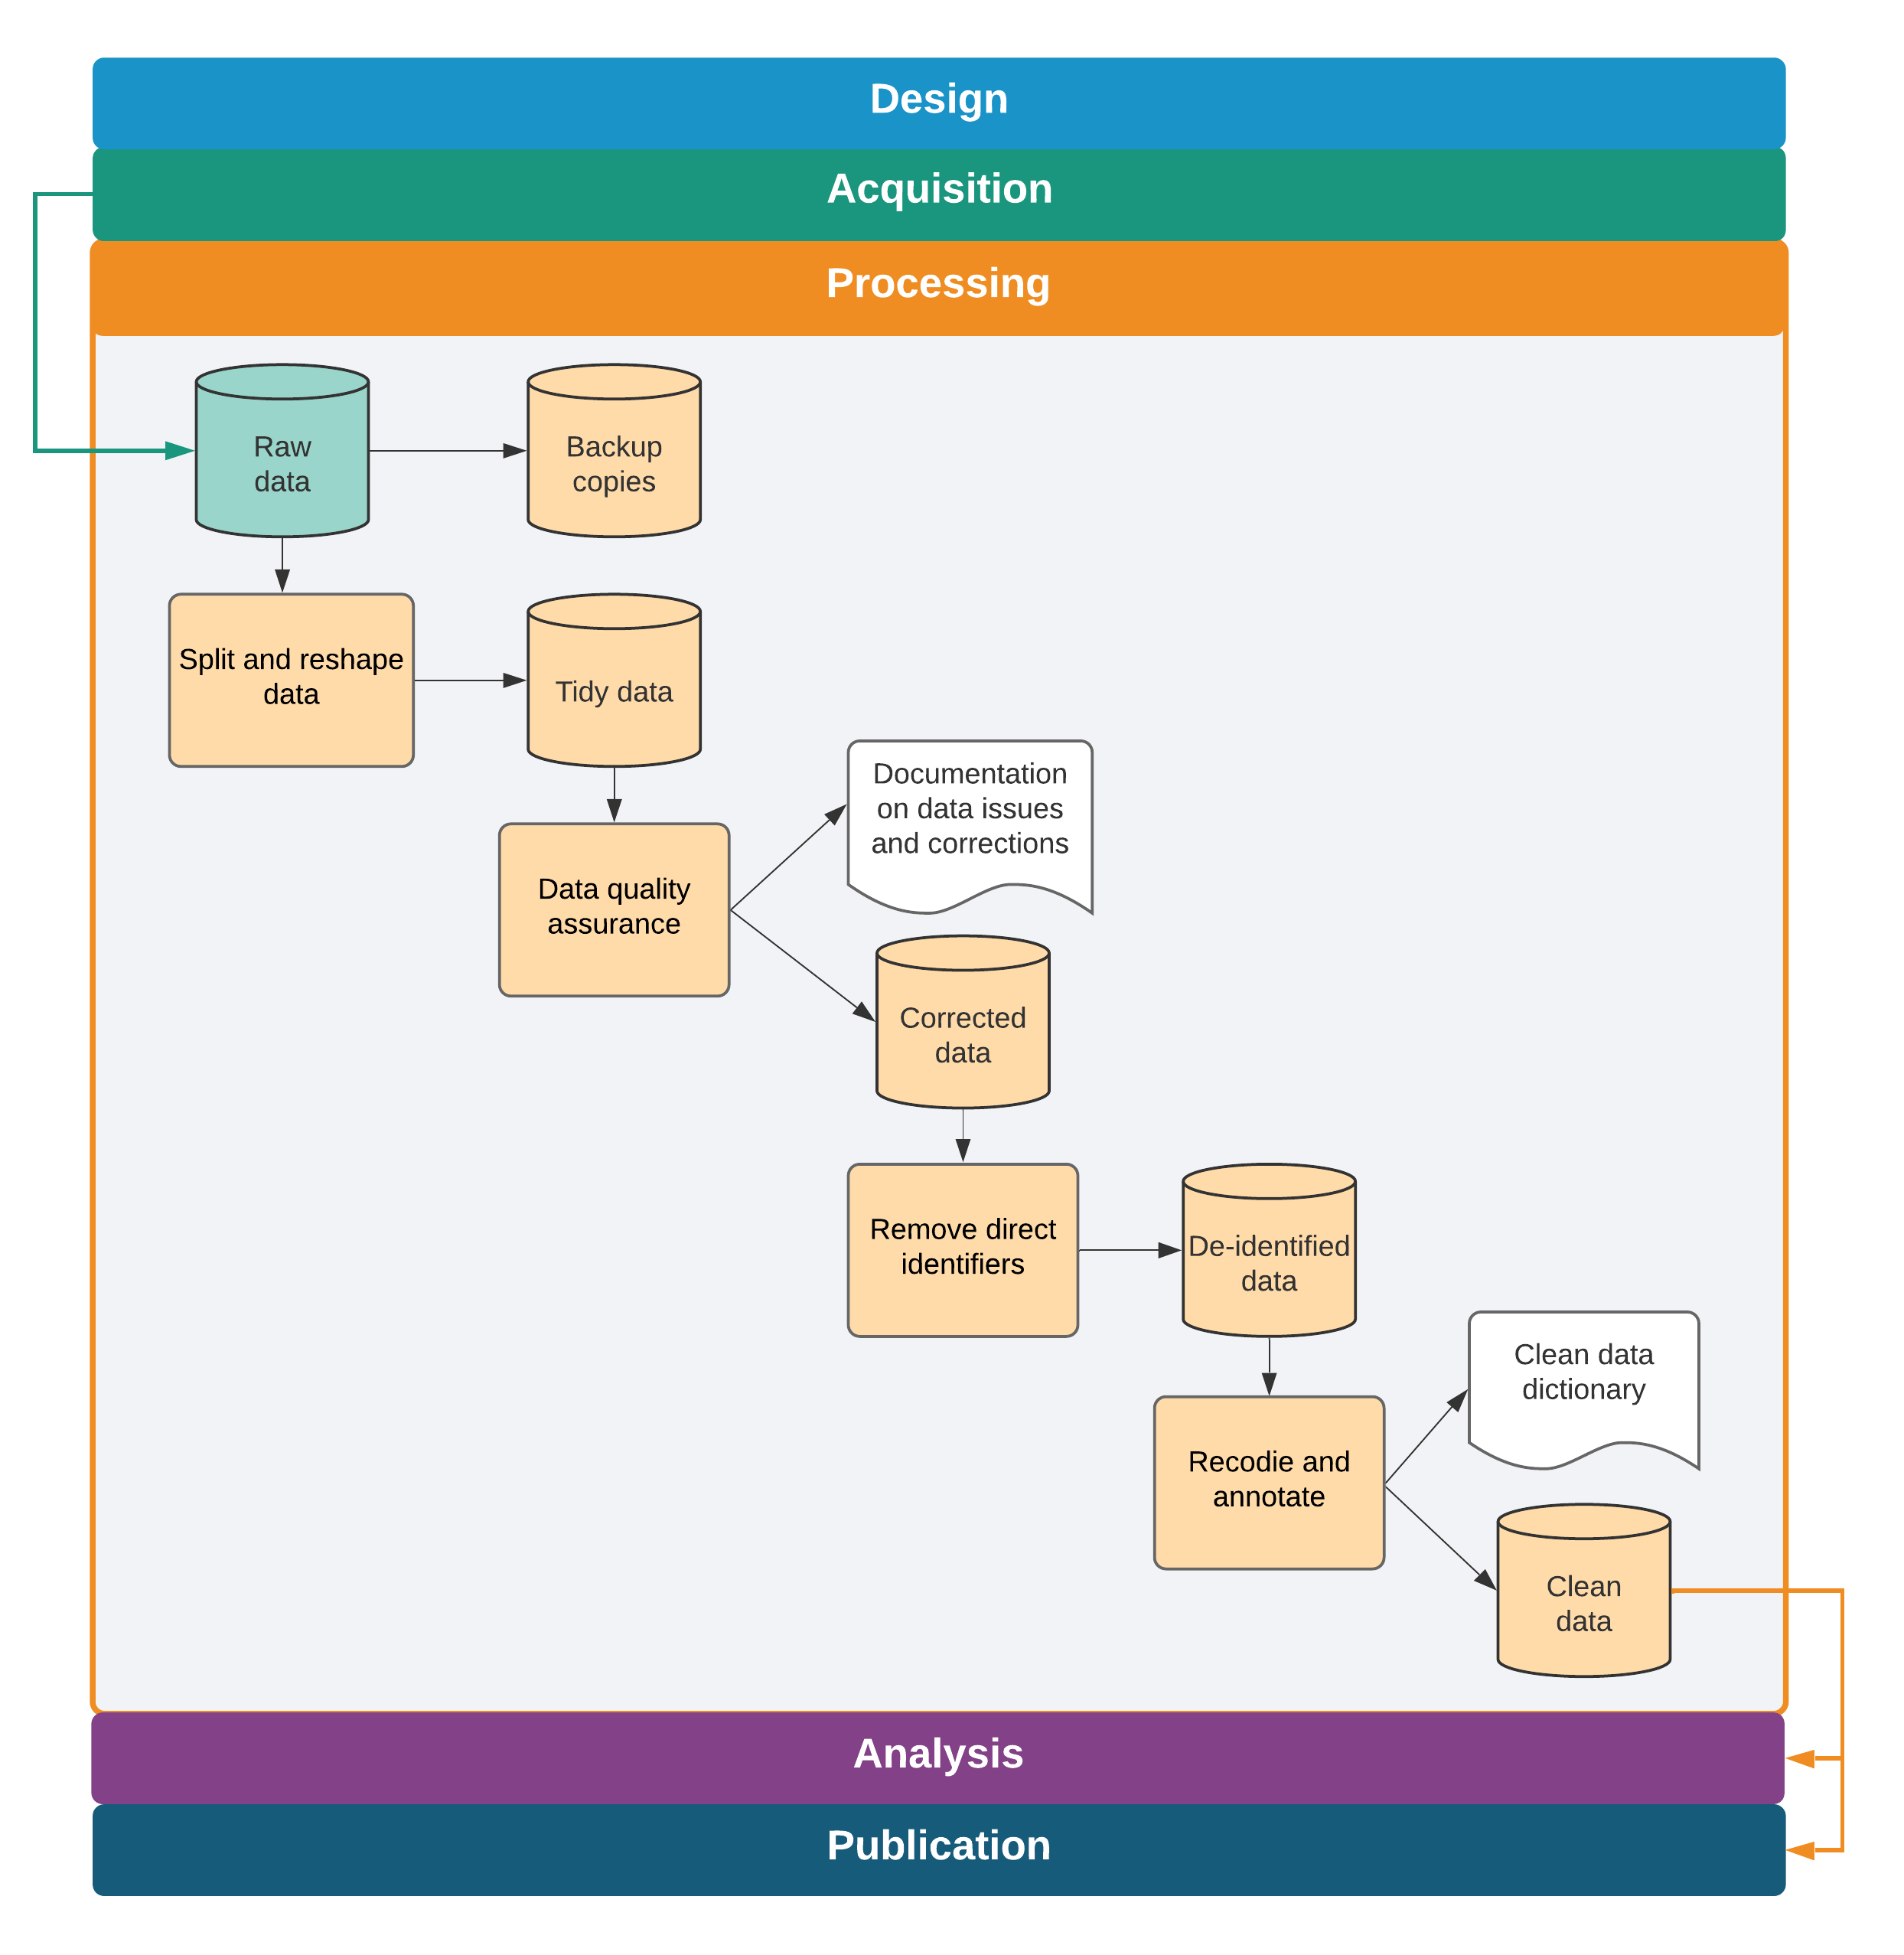
\includegraphics[width=1.6\linewidth]{diagrams/Cleaning}
		\caption{}
		\label{fig:intro}
	\end{figure}
\end{fullwidth}

\subsection{Unique identifiers}

% Uniquely and fully identifying variable
The first step in tidying data is to understand its unit of observation
(what makes a row),
and find out which variable or set of variables is the \textbf{unique identifier}\sidenote{\url{
		https://dimewiki.worldbank.org/ID\_Variable\_Properties}} for each observation in your dataset.
Ensuring that observations are uniquely and fully identified
is arguably the most important step in data cleaning.
It may be the case that the variables expected to be unique identifiers are either incomplete or contain duplicates.
It is also possible for a dataset to have no unique identifier, 
or that the identifier involves a long string that is difficult to work with, such as a full name.
In such cases, cleaning begins by carefully creating a variable that uniquely identifies the data.
Note that while digital survey tools create unique identifiers for each data submission,
that is not the same as having a unique ID variable for each observation in the sample,
as there can be multiple submissions for the same observation.
The unique identifier will be used to link data on observations in one dataset 
with data on the same observations in other datasets, 
such as other rounds of data collection and different data sources.
Therefore, you must keep a canonical dataset of all observations in your data.
This \textbf{master dataset}\sidenote{\url{
		https://dimewiki.worldbank.org/Master\_Data\_Set}}
is discussed in detail in Chapter 3, 
and contains a record of all units ever encountered for each relevant level of observation,
as well as their corresponding unique identifiers.


% Merchand
\texttt{ieduplicates} and \texttt{iecompdup},
two Stata commands included in the \texttt{iefieldkit}
package\index{iefieldkit},\sidenote{\url{https://dimewiki.worldbank.org/iefieldkit}}
create an automated workflow to identify, correct and document
occurrences of duplicate entries.
One advantage of using \texttt{ieduplicates}\sidenote{\url{
		https://dimewiki.worldbank.org/wiki/ieduplicates}} 
to correct duplicated entries is that it creates \textit{duplicates reports}
that record which corrections made and why.
Even if you are not using this command,
it is important to keep a record of all cases of duplicated IDs encountered.

\subsection{Tidying raw data}

Though raw data can be acquired in all shapes and sizes,
development data is most commonly received as one or multiple tables.
Similarly, these tables can organize information in multiple ways,
and not all of them result in easy-to-handle datasets.
Fortunately, a vast literature of database management has identified the format
that makes interacting with the data as easy as it can be.
In database management this is called \textit{normalization},
but when applied to statistics, we call data in such format \textbf{tidy}.\sidenote{\textbf{Tidy data:}
	Datasets where each column represents one variable,
	each row represents one observation, 
	and all variables in a table have the same unit of observation.}
A dataset is tidy when each column represents one variable,\sidenote{\textbf{Variable:} 
	the collection of all data points that measure the same attribute.}
each row represents one observation, 
and all variables in a table have the same unit of observation.
Every other format is \textit{untidy}.
This may seem trivial, but raw data, 
and raw survey data in particular,
is rarely received in a tidy format.
To contribute to the confusion, 
in Stata each column is called a ``variable'', 
and each row an ``observation'',
even though they are not necessarily the same thing.

Every untidy dataset is untidy in its own way,
but the most common case of untidy raw data encountered in development research
are datasets consisting of multiple units of observation stored in the same table. 
If your rows include multiple nested observational units,
having an identifying variable for each row doesn't mean having an identifier for each observation.
Survey data containing nested units of observation is typically 
imported from survey platforms in \textbf{wide format}.\sidenote{\textbf{Wide data:}
	a table where a single variable is divided into multiple columns,
	for example one for each individual in a household.
}
Take, for example, a household survey that includes household-level questions,
as well as a household member roster.
The resulting raw dataset usually consists of a single table
where questions from the household member roster are saved in different columns, 
one for each member, with a corresponding member suffix,
and household-level questions are represented by one column each.
So you have one column called \texttt{ownsmotorcycle},
but a few columns of the format \texttt{gender\_1}, \texttt{gender\_2}, etc.
The data is saved in this format because it's the most efficient way to transfer it:
adding different levels of observation into the same table allows for data to be transferred in a single file.
However, this leads to the widespread practice of interacting with data in wide format for a large part of a project,
although this is not the most efficient way to do so.

To understand how dealing with wide data can be complicated,
just suppose you need to calculate the share of women in your sample using the dataset described above.
The first thing you will need to do is change the format of your table so that each row represents one individual.
Tidy datasets, on the other hand, 
are easier to handle because observations can be aggregated and linked consistently,
without additional steps.
They are also easier to clean, 
as each attribute only needs to be checked once,
as corresponds directly to one question in the questionnaire.

The only example of untidy formats we mentioned so far is wide data,
but as mentioned earlier, there are unlimited ways for data to be untidy.
An alternative example is a table containing information on transactions
and on the firms involved in each transaction.
In this case, the firm-level information will be repeated for all transactions a given firm was involved in.
Analyzing data in this format would give more weight to firms that conducted more transactions,
which may not be consistent with your research design.

The basic process behind tidying a dataset is simple: 
first, you need to identify all the variables that were measured at the same level of observation;
then, create separate tables for each level of observation;
finally, reshape\sidenote{\textbf{Reshape:}
	transform a dataset in such a way that the unit of observation represented by a row changes.} 
the data and remove duplicated rows 
until each table is uniquely and fully identified by the ID variable 
that corresponds to its unit of observation.
In the earlier household survey example,
household-level variables will be stored in one tidy dataset, 
and household-member variables are reshaped to member level and stored in another tidy dataset,
which also contains the household ID for each individual.
So the household ID is intentionally duplicated in the household members table.
In the transaction data example,
the result of the tidying process would be one transaction-level dataset, 
containing variables indicating the ID of all firms involved;
and one firm-level dataset with a single entry for each firm.

Reshaping tables is the most intricate task in this process,
so you should be very familiar with commands such as \texttt{reshape} in Stata and \texttt{pivot} in R.
Another key aspect in this process is to make sure that ID variables are consistent across tables,
so they can always be linked.
There must be a clear way to connect each tidy table to a master dataset.
Note that the tidying process gets more complex as the number of nested groups increases.
That means the steps of identifying the unit of observation of each variable
and reshaping the separated tables need to be repeated multiple times.
However, the more nested groups a dataset includes,
the more efficient it is to deal with tidy data as compared to untidy.
Cleaning and constructing wide datasets, in particular,
is a repetitive and error-prone process.

The next step of data cleaning, data quality monitoring,
may involve comparing different units of observation.
Aggregating sub-units to compare to a higher unit is much easier with tidy data,
which is why we suggest getting your data into a tidy format as early as possible in your workflow. 
If you are conducting primary data collection,
you can start coding the data tidying before the data is acquired,
since you will know in advance in which format it will be received.
In the case of survey data,
tidying datasets will guarantee a one-to-one correspondence
between questions in the questionnaire and columns in the data.
Preparing the data for analysis, the last task in this chapter, 
is much simpler when that is the case. 
 
%------------------------------------------------
\section{Data quality assurance}

% Intro
Whether you are acquiring data from a partner or collecting it directly,
it is important to make sure that data faithfully reflects ground realities.
Although original data typically requires more extensive checks than secondary data,
you should carefully examine and clean any data you are about to use.
When reviewing raw data, you will inevitably encounter data entry mistakes,
such as typos and inconsistent values.
Data quality assurance requires a combination of real-time data checks
and back-checks or validation audits, which often means tracking down
the people whose information is in the dataset.

\subsection{Implementing high frequency quality checks}

% What are HFCs
A key advantage of continuous electronic data intake methods,
as compared to traditional paper surveys and one-time data dumps,
is the ability to access and analyze the data while the project is ongoing.
Data issues can be identified and resolved in real-time.
Designing systematic data checks and running them routinely throughout data intake
simplifies monitoring and improves data quality.
As part of data acquisition preparation,
the research team should develop a \textbf{data quality assurance plan}\sidenote{
	\url{https://dimewiki.worldbank.org/Data\_Quality\_Assurance\_Plan}}.
While data acquisition is ongoing,
a research assistant or data analyst should work closely with the field team or partner
to ensure that the data collection is progressing correctly,
and set up and perform \textbf{high-frequency checks (HFCs)} with the incoming data.

% Why they should be made in real-time
High-frequency checks (HFCs) should carefully inspect key treatment and outcome variables
so that the data quality of core study variables is uniformly high,
and that additional effort is centered where it is most important.
Data quality checks should be run on the data every time it is received from the field or partner
to flag irregularities in the aquisition progress, in sample completeness, or in response quality.
The faster issues are identified, the more likely they are to be solved.
\texttt{ipacheck}\sidenote{
	\url{https://github.com/PovertyAction/high-frequency-checks/wiki}}
is a very useful command that automates some of these tasks,
regardless of the source of the data.

% Completeness
It is important to check continuously that the observations in the data match the intended sample.
In surveys, the software often provides some form of case management features
through which sampled units are directly assigned to individual enumerators.
For data received from partners, this may be harder to validate,
since they are the authoritative source of the data,
so cross-referencing with other data sources may be necessary to ensure completeness of the data.
Even with careful management, it is often the case that raw data includes duplicate or missing entries,
which may occur due to data entry errors or failed submissions to data servers.\sidenote{
	\url{https://dimewiki.worldbank.org/Duplicates_and_Survey_Logs}}
\texttt{ieduplicates}\sidenote{
	\url{https://dimewiki.worldbank.org/ieduplicates}}
provides a workflow for collaborating on the resolution of duplicate entries between you and the provider.
Then, observed units in the data must be validated against the expected sample:
this is as straightforward as merging the sample list with the survey data and checking for mismatches.
Reporting errors and duplicate observations in real time allows the field team to make corrections efficiently.
Tracking data collection progress is important for monitoring attrition,
so that it is clear early on if a change in protocols or additional tracking will be needed.
It is also important to check data collection completion rates
and sample compliance by surveyors and survey teams, if applicable,
or compare data missingness across administrative regions,
to identify any clusters that may be providing data of suspect quality.

% Consistency
High frequency checks should also include content-specific data checks.
Electronic survey and data entry software often incorporate many quality control features,
so these checks should focus on issues survey software cannot check automatically.
As most of these checks are project specific,
it is difficult to provide general guidance.
A retailed knowledge of the questionnaire and a careful examination of the analysis plan
is the best preparation.
Examples include verifying consistency across multiple response fields or data sources,
validation of complex calculations like crop yields or medicine stocks (which require unit conversions),
suspicious patterns in survey timing,
or atypical response patters from specific data sources or enumerators.\sidenote{
	\url{https://dimewiki.worldbank.org/Monitoring_Data_Quality}}
Electronic data entry software typically provides rich metadata,
which can be useful in assessing data quality.
For example, automatically collected timestamps show when data was submitted
and (for surveys) how long enumerators spent on each question,
and trace histories show how many
times answers were changed before or after the data was submitted.

% Following up on flagged issues
High-frequency checks will only improve data quality
if the issues they catch are communicated to the data provider.
There are lots of ways to do this;
what's most important is to find a way to create actionable information for your team.
\texttt{ipacheck}, for example, generates a spreadsheet with flagged errors;
these can be sent directly to the data collection teams.
Many teams choose other formats to display results,
such as online dashboards created by custom scripts.
It is also possible to automate communication of errors to the field team
by adding scripts to link the HFCs with a messaging platform.
Any of these solutions are possible:
what works best for your team will depend on such variables as
cellular networks in field work areas, whether field supervisors have access to laptops,
internet speed, and coding skills of the team preparing the HFC workflows.

\subsection{Conducting back-checks and data validation}

% Conducting back-checks
Careful validation of data is essential for high-quality data.
Since we cannot control natural measurement error
that comes from variation in the realization of key outcomes,
original data collection provides the opportunity to make sure
that there is no error arising from inaccuracies in the data itself.
\textbf{Back-checks}\sidenote{\url{https://dimewiki.worldbank.org/Back\_Checks}} and
other validation audits help ensure that data collection is following established protocols,
and that data is not falsified, incomplete, or otherwise suspect.
For back-checks and validation audits, a random subset of the main data is selected,
and a subset of information from the full survey is
verified through a brief targeted survey with the original respondent
or a cross-referenced dataset from another source (if the original data is not a field survey).
Design of the back-checks or validations follows the same survey design
principles discussed above: you should use the analysis plan
or list of key outcomes to establish which subset of variables to prioritize,
and similarly focus on errors that would be major flags for poor quality data.

% How to implement back-checks
Real-time access to the data massively increases the potential utility of validation,
and both simplifies and improves the rigor of the associated workflows.
You can use the raw data to draw the back-check or validation sample;
this ensures that the validation is correctly apportioned across observations.
As soon as checking is complete, the validation data can be tested against
the original data to identify areas of concern in real-time.
The \texttt{bcstats} command is a useful tool for analyzing back-check data in Stata.\sidenote{
	\url{https://ideas.repec.org/c/boc/bocode/s458173.html}}
Some electronic surveys surveys also provide a unique opportunity
to do audits through audio recordings of the interview,
typically short recordings triggered at random throughout the questionnaire.
\textbf{Audio audits} are a useful means to assess whether enumerators are conducting interviews as expected.
Do note, however, that audio audits must be included in the informed consent for the respondents.


\section{De-identifying research data}

Up to this point, you were probably handling confidential data.
This is due to the fact that effective data quality monitoring
frequently requires you to identify the individual observations in your dataset,
and the people who acquired information about them.
Having this data will allow you to quickly follow up on issues identified,
and verify what caused them.
Handling confidential data such as \textbf{personally-identifying information}\index{
	personally-identifying information}
requires a secure environment and often involves
decrypting data before accessing it.
De-identifiying the data simplifies this workflow and reduces the risk of harmful leaks.
This section describes how to perform de-identification of data 
to be shared within a research team and with a wider audience.

\subsection{Protecting privacy as a researcher}

% Dealing with human subjects
Most of the field research done in development involves human subjects.\sidenote{
	\url{https://dimewiki.worldbank.org/Human_Subjects_Approval}}
\index{human subjects}
As a researcher, you may have access to personal information about your subjects:
where they live, how rich they are, whether they have committed or been victims of crimes,
their names, their national identity numbers, and other sensitive data.
PII data carries strict expectations about data storage and handling,
and it is the responsibility of the research team to satisfy these expectations.\sidenote{
	\url{https://dimewiki.worldbank.org/Research\_Ethics}}
Your funder or employer will most likely require you to hold a certification from a source
such as Protecting Human Research Participants\sidenote{
	\url{https://phrptraining.com}}
or the CITI Program;\sidenote{
	\url{https://about.citiprogram.org/en/series/human-subjects-research-hsr}}
and your team will need to present a plan to handle data securely for IRB approval.

% Options for dealing with PII data: only collect it if extremely necessary, encrypt it, restrict access, de-identify it
In general, though, you shouldn't need to handle PII data very often
once data collection is completed.
You can take simple steps to avoid risks by minimizing the handling of PII.
First, only collect information that is strictly needed for the research.
Second, avoid the proliferation of copies of identified data.
There should never be more than one copy of the raw identified dataset in the project folder,
and it must always be encrypted.
Even within the research team,
access to PII data should be limited to team members who require it for their specific tasks.
Data analysis that requires identifying information is rare
and in most cases can be avoided by properly linking masked identifiers to research information
such as treatment statuses and weights, then removing unmasked identifiers.

% De-identification vs anonymization
Therefore, once data is securely collected and stored,
the first thing you will generally do is \textbf{de-identify} it,
that is, remove direct identifiers of the individuals in the dataset.\sidenote{
	\url{https://dimewiki.worldbank.org/De-identification}}
\index{de-identification}
Note, however, that it is in practice impossible to \textbf{anonymize} data.
There is always some statistical chance that an individual's identity
will be re-linked to the data collected about them
-- even if that data has had all directly identifying information removed --
by using some other data that becomes identifying when analyzed together.
For this reason, we recommend de-identification in two stages.
The \textbf{initial de-identification} process strips the data of direct identifiers
as early in the process as possible,
to create a working de-identified dataset that
can be shared \textit{within the research team} without the need for encryption.
This simplifies workflows.
The \textbf{final de-identification} process involves
making a decision about the trade-off between
risk of identifying individuals and the utility of the data
before publicly releasing a dataset.\sidenote{
	\url{https://sdcpractice.readthedocs.io/en/latest/SDC\_intro.html\#need-for-sdc}}
The following section describes how to implement these processes.


\subsection{De-identification in practice}

% Initial de-identification
To simplify workflows, the data should be de-identified as early as possible.
Once you create a de-identified version of the dataset,
you no longer need to interact directly with the encrypted raw data.
Note that if the raw data contained different units of observation,
at this point your dataset should consist of set of tidy tables.
In this case, each of them needs to be de-identified separately, but
the workflow will be the same for all of them.

During the initial round of de-identification, 
datasets must be stripped of personally identifying information.\sidenote{
	\url{https://dimewiki.worldbank.org/De-identification}}
To do so, you will need to identify all variables that contain
such information.\sidenote{\url{
		https://www.povertyactionlab.org/sites/default/files/resources/J-PAL-guide-to-deidentifying-data.pdf}}
For data collection, where the research team designs the survey instrument,
flagging all potentially identifying variables at questionnaire design stage
simplifies the initial de-identification process.
If you did not do that, or you received original data by another means,
there are a few tools to help flag variables with personally-identifying data.
JPAL's \texttt{PII-scan} and
IPA's \texttt{PII\_detection}\sidenote{
	\url{https://github.com/PovertyAction/PII\_detection}}, 
scan variable names and labels for common string patterns associated with identifying information.\sidenote{
	\url{https://github.com/J-PAL/PII-Scan}}
The World Bank's \texttt{sdcMicro}
lists variables that uniquely identify observations, 
but it is less efficient for large datasets.\sidenote{
	\url{https://sdctools.github.io/sdcMicro/articles/sdcMicro.html}}
The \texttt{iefieldkit} command \texttt{iecodebook}
lists all variables in a dataset and exports an Excel sheet
where you can easily select which variables to keep or drop.\sidenote{
	\url{https://dimewiki.worldbank.org/Iecodebook}}

% Initial de-identification in practice
Once you have a list of variables that contain confidential information,
assess them against the analysis plan and first ask yourself for each variable:
\textit{will this variable be needed for the analysis?}
If not, the variable should be dropped.
Don't be afraid to drop too many variables the first time,
as you can always go back and remove variables from the list of variables to be dropped,
but you can not go back in time and drop a PII variable that was leaked
because it was incorrectly kept.
Examples include respondent names and phone numbers, enumerator names, taxpayer 
numbers, and addresses.

For each confidential variable that is needed in the analysis, ask yourself:
\textit{can I encode or otherwise construct a variable that masks the confidential component, and
	then drop this variable?}
This is typically the case for most identifying information.
Examples include geocoordinates
(after constructing measures of distance or area,
drop the specific location)
and names for social network analysis (can be encoded to secret and unique IDs).
If the answer to either of the two questions above is yes,
all you need to do is write a script to drop the variables that are not required for analysis,
encode or otherwise mask those that are required,
and save a working version of the data.
If confidential information is strictly required for the analysis itself and cannot be
masked or encoded,
it will be necessary to keep at least a subset of the data encrypted through
the data analysis process.

% Final de-identification: sdcMicro
After the this step, your dataset will consist of one or multiple tidy, 
de-identified tables.
This is the underlying source for all cleaned and constructed data,
the dataset that you will interact with directly during the remaining tasks described in this chapter.
Because identifying information is typically only used during data collection,
when teams need to find and confirm the identity of interviewees,
de-identification should not affect the usability of the data.
However, access to this data should still be restricted to the research team only,
as it's possible that combining a group of variables,
or taking into account information that is not the dataset,
may lead to the identification of the individuals in the sample.
It is common, and even desirable, for teams to make data publicly available
once the tasks discussed in this chapter are concluded.
This will allow other researchers to conduct additional analysis and to reproduce your finding.
Before that can be done, however,
you should further consider whether your data can be re-identified,
in a process we call \textbf{final de-identification},
which will be discussed in more detail in chapter \ref{ch:7}.


\section{Preparing data for analysis}

% What is data cleaning
The last step in the data cleaning process involves
making the dataset easy to use and understand, and 
carefully exploring each variable to document their distributions 
and identify patterns that may bias the analysis.
The resulting dataset will contain only the variables collected in the field, and
no modifications to data points will be made, 
except for corrections of mistaken entries.
You may have more tables in your dataset now then originally received,
and they may have a different \textit{format},
but the information contained is still the same.
Apart from the \textbf{cleaned dataset} (or datasets) itself,
cleaning will also yield extensive documentation describing  it.

% Section overview
During data cleaning, you will acquire in-depth understanding of the contents and structure of your data.
This knowledge will be key to correctly construct final indicators and analyze them.
So don't rush through this step.
It is common for cleaning to be the most time-consuming task in a project.
In this section, we will introduce some concepts and tools to make it more efficient and productive.
The section is separated into three topics:
exploring the data, making corrections, and recoding and annotating.
They are separated here because they are different in nature.
In practice, however, they are all done at the same time.


\subsection{Getting to know your data}

% What to look for when exploring the data
The first time you interact with your data is during quality checks.
However, these checks are often programmed before you receive all the data.
Furthermore, because quality checks are usually time-sensitive, 
there may not be time to explore the data at length.
During data cleaning, on the other hand, 
you will need to inspect each variable closely.
Use tabulations, summary statistics, histograms and density plots to understand the structure of data,
and look for patterns or irregularities.
Think critically about what you see:
are the values shown consistent with the information the variable represents?
How do distributions look? 
Are there any outliers or missing values?
Could distributional patterns be caused by data entry errors?
Are related variables consistent with each other?

% Document patterns rather than fix them
At this point, it is more important to document your findings
than to try to address any irregularities found.
There is a very limited set of changes that should be made to the raw data during cleaning.
They are described in the next two sections,
and are usually applied to each variable as you explore them.
Most transformation resulting in data points that were not directly observed in the original data
will be done during \textbf{construction}, a process discussed in the next chapter.
For now, focus on creating a record of what you observe,
extensively documenting the data being explored.
You will use this documentation when discussing with your team
how to address irregularities when you get to the construction stage.
This material will also be valuable during exploratory data analysis.

\subsection{Correcting data points}

% Correct or not correct
As mentioned earlier, 
corrections to issues identified during data quality monitoring are
the only changes done to individual data points during the data cleaning stage.
However, there is a lot of discussion about whether one should modify such data points at all.
Some argue that follow-ups to the issues identified are costly and add limited value.
Since it is not possible to check each and every possible data entry error,
doing so can create a false sense of security from issues identified on a few main variables. 
Additionally, manually inspected data may suffer from considerable inspector variability.
Therefore, there's an argument for using data quality monitoring tools
as a tool to detect completely fraudulent observations and
revisiting data collection protocols or decisions.
On the other hand, there is also an argument to be made
against keeping clear typing errors that have been found or for
collecting data about mistakenly skipped survey modules.

% Documentation
Whether you decide to modify your data or not,
a careful record of which data entry mistakes were identified.
If no data points are modified, 
it may still be helpful to add flags to observations containing
potentially problematic values,
so you can verify how they affect results during analysis.
If your team decides to follow up on these issues and 
try to determine what the correct value is,
the follow-up process must also be thoroughly documented.
Be very careful not to include confidential information in documentation that is not securely stored,
or that you intend to release as part of a replication package or data publication.
Finally, remember not to make changes directly to the raw data.
Instead, any corrections must be done as part of data cleaning,
and saved to a new dataset.

\subsection{Recoding and annotating data}

% Why recoding and annotating data are important
The cleaned dataset is the starting point of data analysis.
It will be extensively manipulated to construct analysis indicators,
so it is important for it to be easily processed by statistical software.
To make the analysis process smoother, 
anyone opening it for the first time should have all the information needed to interact with it,
even if they were not involved in the acquisition or cleaning process.
This will save them time going back and forth between the dataset and its accompanying documentation. 

% Encoding variables
Often times, datasets are not imported into statistical software in the most efficient format.
The most common example is string (text) variables:
categorical variables and open-ended responses are often read as strings.
However, variables in this format cannot be used for quantitative analysis.
Therefore, categorical variables must be transformed into other formats,
such as \texttt{factors} in R and \texttt{labeled integers}\sidenote{\url{https://dimewiki.worldbank.org/wiki/Data\_Cleaning\#Value\_Labels}} in Stata.
Additionally, open-ended responses stored as strings usually have a high risk of being identifiers, 
so cleaning them requires extra attention.
The choice names in categorical variables
(called \textit{value labels} in Stata and \textit{levels} in R)
should be accurate and concise, 
and link directly to the data collection instrument.
Adding choice names to categorical variables 
makes it easier to understand your data as you explore it,
and thus reduces the risk of small errors making their way through into the analysis stage.

% Recoding missing values
In survey data, it is common for non-responses such as ``Don't know'' and ``Declined to answer''
to be represented by arbitrary survey codes. 
The presence of these values could bias your analysis,
since they don't represent actual observations of an attribute.
They need to be turned into \textit{missing values}.
However, the fact that a respondent didn't know how to answer a question is also useful information
that would be lost by simply omitting all information.
In Stata, this information can be elegantly conserved using extended missing values.\sidenote{
	\url{https://dimewiki.worldbank.org/Data\_Cleaning\#Survey\_Codes\_and\_Missing\_Values}}

% Labeling variables
We recommend that the cleaned dataset be kept as similar to the raw data as possible.
This is particularly important regarding variable names:
keeping them consistent with the raw data makes data processing and construction more transparent.
Unfortunately, not all variable names are informative.
In such cases, one important piece of documentation,
the variable dictionary, makes the data easier to handle.
When a data collection instrument is available, 
it is often the best dictionary one could ask for.
But even in this cases, going back and forth between files can be inefficient,
so annotating variables in a dataset is extremely useful.
In Stata, \textit{variable labels}\sidenote{\url{
	https://dimewiki.worldbank.org/wiki/Data\_Cleaning\#Variable\_Labels}} must always be present in a cleaned dataset.
They should include a short and clear description of the variable.
A lengthier description, that may include, for example,
the exact wording of a question, may be added through \textit{variable notes}.
In R, it is less common to use variable labels,
and a separate dataset with a variable dictionary is often preferred,
but \texttt{dataframe attributes} can be used for the same purpose.

% Dropping irrelevant variables
Finally, any information that is not relevant for analysis may be removed from the dataset.
In primary data, it is common to collect information for quality monitoring purposes,
such as notes, duration fields and surveyor IDs.
Once you are past the quality monitoring phase,
these variables may be removed from your dataset.
In fact, to make the data easier to handle,
you may choose to start from a minimal set of variables,
and add new ones as you clean them.
To make sure the cleaned dataset file doesn't get too big to be handled,
use commands such as \texttt{compress} in Stata to make sure the data
is always stored in the most efficient format.

% Cleaning tools: iecodebook, tidyverse
Although all these tasks are key to making the data easy to use,
implementing them can be quite repetitive and create convoluted scripts.
The \texttt{iecodebook} command suite, part of the \texttt{iefieldkit} Stata package,
is designed to make some of the most tedious components of this process more efficient.\sidenote{
	\url{https://dimewiki.worldbank.org/iecodebook}}
\index{iecodebook}
It also creates a self-documenting workflow,
so your data cleaning documentation is created alongside that code,
with no extra steps.
As far as we know, there are no similar resources in R.
However, the \texttt{tidyverse}\sidenote{\url{https://www.tidyverse.org/}} packages
compose a consistent and useful grammar to perform the same tasks.


\subsection{Documenting data cleaning}
Throughout the data cleaning process,
you will often need extensive inputs from the people responsible for data collection.
(This could be a survey team, the government ministry responsible for administrative data systems,
the technology firm that generated remote sensing data, etc.)
You should acquire and organize all documentation of how the data was generated, such as
reports from the data provider, field protocols, data collection manuals, survey instruments,
supervisor notes, and data quality monitoring reports.
These materials are essential for data documentation,\sidenote{
	\url{https://dimewiki.worldbank.org/Data\_Documentation}}
\index{Documentation}
and should be stored alongside your data dictionary and codebooks.
You will probably need these files during analysis,
and they should be published along with the data,
so other researchers may use them for their analysis as well.

Once you have a cleaned, de-identified dataset and the documentation to support it,
you have created the first research output of your project: a dataset.
Chapter 7 will get into the details of data release.
For now, all you need to know is that your team 
should consider submitting this dataset for publication,
or at least archiving and cataloguing,
even if it will remain embargoed for some time.
This will help you organize your files and create a backup of the data,
and some donors require that the data be filed as an intermediate step of the project.

%--------------------------------------------------------------
